\documentclass[../primer.tex]{subfiles}

\begin{document}

\chapter{Sensitivity Analysis}

\section{Motivation} \label{sec:orgdc914a7}
Here at Stanford,\footnote{Circa 2018} we host the Predictive Science Academic
Alliance Program II
(\href{http://exascale.stanford.edu/content/stanford-psaap-ii-motivation-1}{PSAAP
  II}). This project is motivated by a solar receiver intended for green energy
production, with heat transfer enhanced via a particle-laden working fluid. This
is a system of enormous complexity, featuring particle-laden turbulent flow with
radiative heat transfer. The difficulty arises (in part) due to the complex
multiphysics, which necessitates careful modeling for computational
tractability. For example, the Stanford PSAAP II simulation codes implement
models not just for the turbulence, but also novel models for radiation
transport, accounting for distributed particles smaller than the resolved
gridsize.

\begin{figure}[!ht]
  \centering
  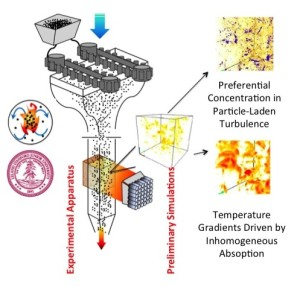
\includegraphics[width=0.75\textwidth]{./images/psaap}
  \caption{Schematic for the PSAAP II physical problem. This graphic
    highlights some of the complex interactions between traditionally
    separate domain physics. The complexity of the physics necessitates
    modeling assumptions, which introduce uncertainties.}
  \label{fig:psaap}
\end{figure}

\marginnote{Note that some of the techniques we will discuss are
sample-intensive. Most of the techniques described below are intended for
\emph{computer experiments}; that is, simulation campaigns run on computer codes.
Contrast these with \emph{physical experiments}, in which the physical
world `solves' the equations of motion automatically.}

\clearpage

These modeling assumptions introduce non-physical coefficients, which constitute
additional uncertainties in the problem. Table \ref{tab:uncertainties} lists
these and other examples of uncertainties in the PSAAP II problem. For practical
purposes, we would be interested in how \emph{all} the uncertainties affect practical
output quantities of interest, such as the device efficiency. If the results
were largely insensitive to our uncertainties over a range of physically
relevant values, this would build confidence in our ability to perform accurate
simulations, and would potentially enable the design of novel solar receivers.

\begin{table}[!ht]
\caption{A non-exhaustive list of examples of uncertainties
in the Stanford PSAAP II problem.}
\label{tab:uncertainties}
\begin{tabular}{@{}ll@{}}
Type                       & Source                        \\
\hline
Input Uncertainties        & Turbulence model parameters   \\
Model Discrepancies        & Limitations of eddy viscosity \\
Numerical Errors           & Artificial dissipation        \\
Experimental Uncertainties & Probe accuracy limitations    \\
\end{tabular}
\end{table}

If our outputs were \emph{not} insensitive to these uncertainties, that would signal
that we need to either reduce the uncertainties (say through experimentation),
or account for the uncertainties in our results (say through uncertainty
propagation). This would necessitate a combination of experimental and
computational work -- both are expensive activities.

This expense is compunded by the \emph{curse of dimensionality}, which states
(roughly) that the expense of a procedure\footnote{e.g. a parameter study, or
numerical quadrature} tends to grow \emph{exponentially} with dimension. Not only is
gathering data expensive; we need many data points to understand
high-dimensional parameter spaces!

\begin{figure}[htbp]
\centering
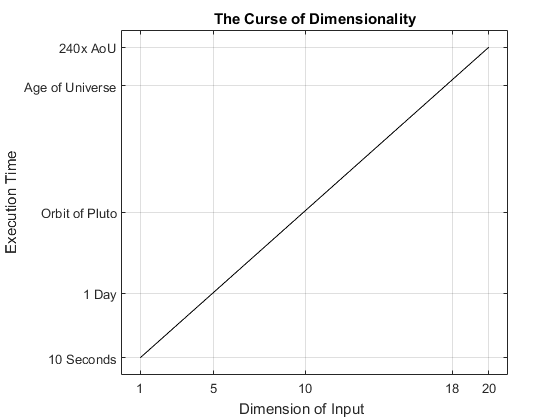
\includegraphics[width=.9\linewidth]{./images/curse_of_dimensionality.png}
\caption{Cartoon depicting computational expense under the curse of dimensionality. Imagine that we are performing quadrature (numerical integration), and are using a simple tensor-product approach; i.e. using 10 evaluations per dimension. If a computer implementation of our qoi evaluates in one second, it will take 10 seconds to study a 1-dimensional function. For a 5-dimensional function, this will take a day to evaluate. This exponential growth quickly grows out of hand, reaching an execution time of nearly the Age of the Universe at just 18 dimensions.}
\end{figure}

Ideally, one would like to know which parameters are most influential,
preferably before embarking on an expensive simulation campaign. This is the
insight that sensitivity analysis seeks to provide. A sensible way to address
this curse is to attack dimensionality directly -- to reduce the number of input
parameters. As a simple approach, we could perform a sensitivity analysis,
identify those parameters which do not appreciably affect our qoi, and freeze
them to nominal values. This effectively reduces the dimensionality of the
problem, ameliorating the curse of dimensionality.

\subsection{An intermediate conclusion}
\label{sec:org6367ab6}
Sensitivity analysis is about determining how input parameters affect a chosen
quantity of interest. We would apply these results at multiple stages in an
analysis. A sensitivity analysis could help identify which uncertainties are
worth characterizing through a physical experiment. Such an analysis could
also identify parameters which can be frozen to nominal values, making further
computational experiments less expensive.

\section{Local vs Global}
\label{sec:org4eb0133}
There are two broad philosophies to sensitivity analysis: local and global.
Local sensitivity generally refers to studying the gradient of a qoi; the
derivative (partial or total) of the output qoi with respect to its input
parameters, computed at a set of nominal values. Global sensitivity generally
refers to variance contributions; the amount of variance exhibited in the output
qoi, as contributed by different sets of the input parameters.

\begin{figure}[!ht]
  \centering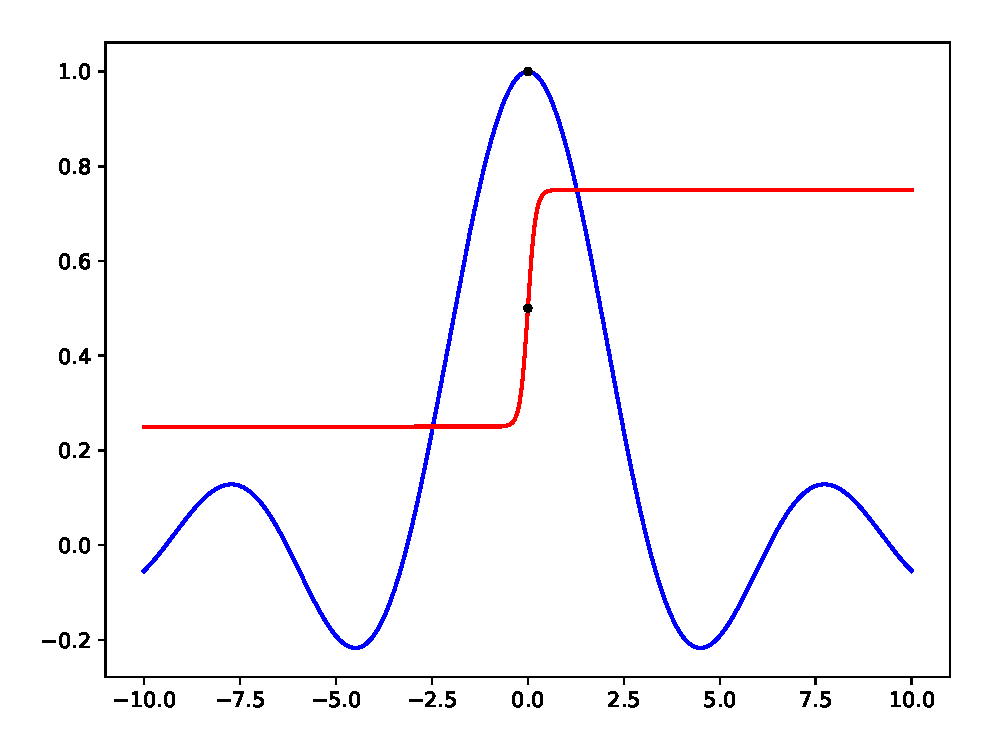
\includegraphics[width=0.75\textwidth]{./images/ex1}
  \caption{Cartoon functions to depict differences between local and global
  sensitivity. The vertical axis corresponds to our qoi, while the horizontal
  corresponds to an input parameter. The black dot is the point of interest
  for local sensitivity. The blue curve has a great deal of global sensitivity,
  but zero local sensitivity. The red curve has comparatively little global
  sensitivity, but a large local sensitivity. Which metric is important
  depends on the objective of the study.}
  \label{fig:ex1}
\end{figure}

As implied by the names, the two approaches give different pieces of
information. Depending on the context, one or the other may be the `right'
metric to study. Figure \ref{fig:ex1} provides a simple cartoon illustration of
two cases where local and global sensitivities will be in disagreement.

In what follows, we will focus on local sensitivity, and leave global
sensitivity to a following set of notes.

\section{Preliminary Considerations}
\label{sec:org797e9af}
Before we jump into computing the derivative, we will first discuss some
preliminary concerns. Before computing the derivative, we ought to determine
\emph{where} we ought to evaluate! Furthermore, we ought to have some clear goal in
mind of what to \emph{do} with the gradient before we set out to compute it.

To introduce some notation, let \(f(\vx):\R{d}\to\R{}\) be our quantity of
interest (qoi), and let \(\Omega\subseteq\R{d}\) be the parameter space of
interest. The first object we'll study is \(\Omega\).

\subsection{Region identification}
\label{sec:orgcd17394}
The parameter space \(\Omega\) may itself be uncertain, or at least poorly
characterized. It is possible that insights gained in one subset of \(\Omega\) may
not hold in other regions, or modeling choices which are appropriate in one
region may fail in another. Figure \ref{fig:moody} depicts a classical example
from fluid mechanics where physical behavior changes dramatically in different
regions of parameter space. The punchline here is that one should think
carefully about the domain \(\Omega\) to be studied, as this will affect the
conclusions drawn from sensitivity analysis, either local or global.

\begin{figure}[!ht]
  \centering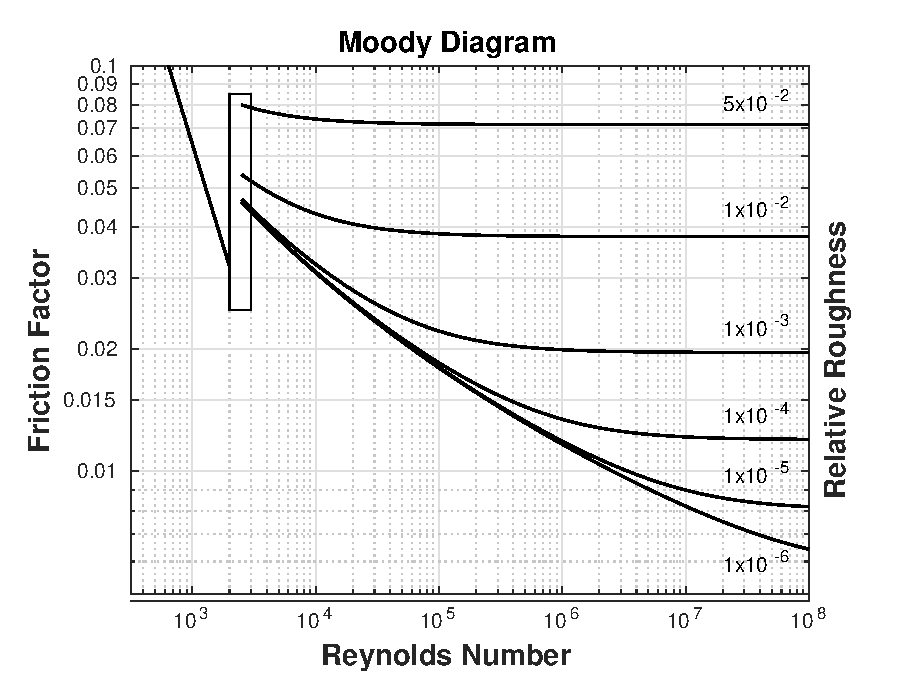
\includegraphics[width=0.75\textwidth]{./images/moody_diagram}
  \caption{The Moody Diagram depicts the dimensionless pressure losses (Friction Factor)
  against relevant dimensionless parameters. Note that the Relative Roughness only
  becomes relevant at high Reynolds Number. This sort of information would not be
  discovered through a global sensitivity analysis, and instead requires careful
  probing of local properties.}
  \label{fig:moody}
\end{figure}

\subsection{Pseudoglobal approach}
\label{sec:orge4ebe04}
Studying the gradient at every point in parameter space is both expensive and
conceptually challenging in high dimensions. Visually inspecting a high
dimensional space is not possible, and generally requires some form of dimension
reduction for visualization.

One could generate a summary of local behavior by computing an expectation of
the gradient, for example

\begin{equation}\label{eq:grad-avg}
  \E\left[\left|\frac{\partial f}{\partial x_i}\right|\right],
\end{equation}

\noindent which can be approximated via Monte Carlo sampling.\footnote{Monte Carlo is
a technique for approximating integrals, which can be viewed as expectations
against some integral weight, possibly uniform. One proceeds by drawing samples
\(\vx_i\sim\rho\) according to the integral weight, and estimating
\(\E[f(\vx)]\approx\frac{1}{n}\sum f(\vx_i)\).} This quantity could be considered
a global average of local effects, mixing the two philosophies. The textbook
(Ch. 6) describes this as a \emph{pseudoglobal} approach. \Cref{eq:grad-avg} is
closely related to \emph{Morris screening}, a global sensitivity approach we will
discuss in the next set of notes, and is also discussed in Chapter 15 of the
textbook.\cite{smith2013uncertainty}

\marginnote{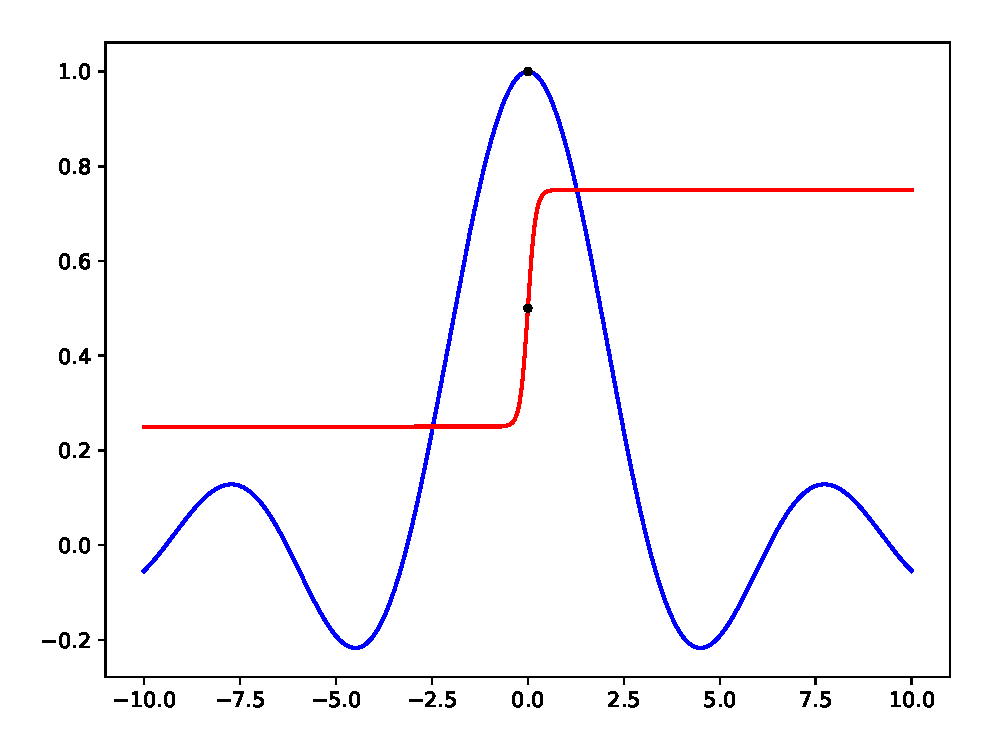
\includegraphics[]{./images/ex1}}

If \eqref{eq:grad-avg} were small for some set of indices
\(I\subseteq\{1,\dots,d\}\), we could freeze the associated variables to nominal
values \(\vx_{I}=\vx_{I,\text{Nom}}\). This would reduce the dimensionality of the
problem. Note that a purely local approach would \emph{not} endorse this
pick-and-freeze approach, as illustrated by the blue curve in Figure
\ref{fig:ex1}, repeated in the margin. Furthermore, this pseudoglobal approach
is prone to miss nonlinear behavior in the function -- imagine if we had sampled
outside the sharp region of the red curve in Figure \ref{fig:ex1}. A
pseudoglobal approach is not necessarily the best way to attack the problem of
freezing variables; this is better handled via global sensitivity analysis.

\subsection{Determining the stability of an optimal point}
\label{sec:org26d8e84}
Unconstrained optimization is conceptually straightforward; critical points are
found where the gradient of the qoi is zero. Optimal points are then found where
the curvature meets an additional criterion.\footnotemark The magnitude of the
curvature gives some sense of how sensitive the optimal point is to changes in
parameter values.

\footnotetext{e.g. for a maximum, we want negative curvature}

For constrained optimization, the intuition is slightly different. Rather than
having zero gradient, a function must meet a stationarity condition; its
gradient must `balance' that of the constraints.\footnote{More formally, the
Karush-Kuhn-Tucker (KKT) conditions give a set of first-order necessary
conditions for optimality.} Figure \ref{fig:opt} gives a cartoon example of a
constrained optimization problem. The punchline is that the gradient of our qoi
need not be zero for a constrained optimal point. This is not a big deal if our
parameters are known exactly.

\begin{figure}[!ht]
  \centering
  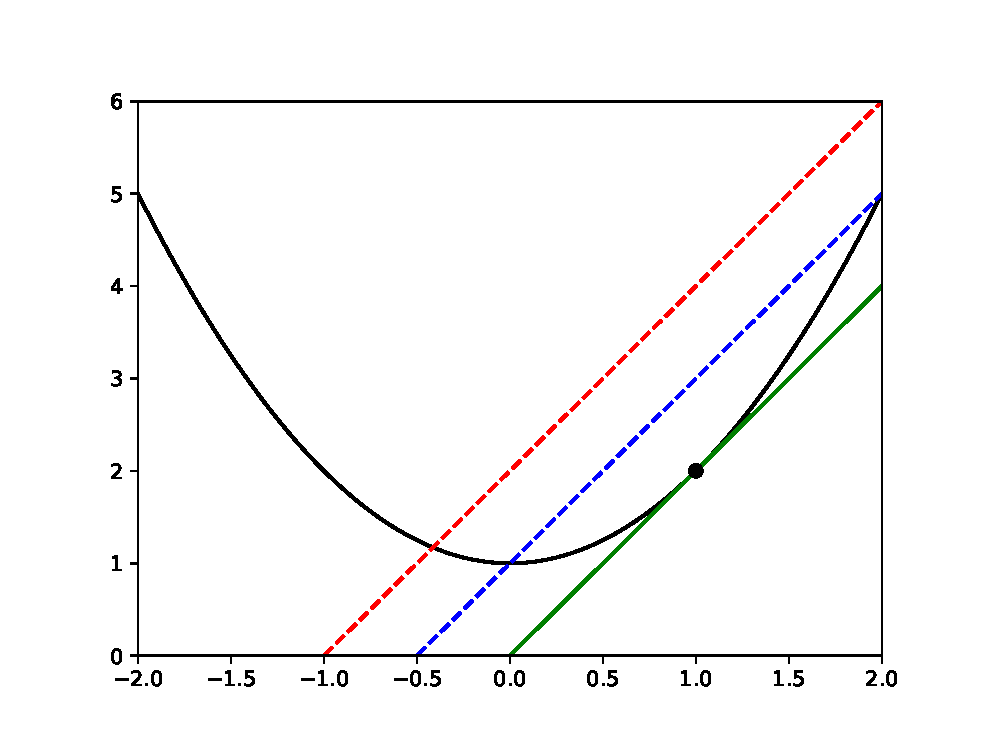
\includegraphics{./images/ex2}
  \caption{Cartoon of constrained optimization: The black curve is the
    constraint, while the red, blue, and green lines are isocontours of
    the qoi. If the gradient of our qoi is not aligned with the gradient
    of the constraint at their intersection -- if they are not \emph{tangent}
    -- then one can find an improved function value by sliding along the
    constraint. Here, the green isocontour is tangent at the black dot,
    which corresponds to an optimal point. The gradient of the qoi is
    nonzero at this point; if there is uncertainty in the input parameters,
    this could lead to the realized value of the response being significantly
    less than desired. One may quantify these effects through local sensitivity
    analysis}
  \label{fig:opt}
\end{figure}

However, if our parameters are uncertain, a nonzero gradient provides some
information about how much this uncertainty can affect our optimal value. As a
more concrete example in an engineering design context, one could do a Taylor
approximation to determine how much the qoi may fluctuate, then add margin to
the design to account for this uncertainty.

\section{Finite Differencing}
\label{sec:org90b543e}
Conceptually, approximating the derivative is quite simple. One simply chooses a
base point \(\vx\) and considers a finite step-size \(\Delta x\) approximation to
the derivative\footnote{Note that this is the \emph{partial derivative}, which is
usually denoted with \(\partial\). We're going to reserve the \(\partial\) symbol
for a different operation in these notes.}

\begin{equation}
  \frac{df}{dx_i} \approx \frac{f(x_1,\dots,x_i+\Delta x,\dots,x_d) - f(\vx)}{\Delta x}.
\end{equation}

However, there are some complications with this approach. First, this
computational procedure requires additional evaluations, with a cost that grows
linearly with dimensionality \(d\). If we require \(N\) evaluations of the gradient
for a desired procedure (e.g. building a map of the gradient or performing
quadrature), then our total cost will be \(O(Nd)\).

The other complication is choosing a sensible \(\Delta x\). Recent work has
studied the selection of \(\Delta x\) based on measuring the \emph{empirical noise} of
a function; that is, tailoring the step-size based on the observered variability
in a computed qoi arising from a computational procedure.\cite{more2012}

\section{Adjoint Method}
\label{sec:org39314ad}
The adjoint is clever method for cheaply computing the sensitivity of a scalar
qoi. This is particularly useful if evaluating our qoi requires solving some
parameterized governing equation \(F(\vy,\vx)\) for a state variable (e.g. flow
field) on which our qoi depends \(f(\vy,\vx)\). Practically, it allows us to
compute the total derivative of our qoi \(\frac{df}{d\vx}\) at the expense of one
additional solution comparable to \(F(\vy,\vx)\). Steven Johnson \cite{johnson2012}
has some very nice introductory notes on the topic, which I follow for the next
example. He also points to a paper by Cao et al.\cite{cao2003adjoint} which gives
a more general treatment of the adjoint.

\subsection{Example: Linear System}
\label{sec:org3c66c8a}
The spirit of the adjoint method is well-illustrated by a simple linear system.
Suppose we have a governing equation for the state \(A_{jk}(\vx)y_k=b_j(\vx)\)
\footnote{I'm going to use \href{https://en.wikipedia.org/wiki/Einstein\_notation}{Einstein notation} here to help make this easier to
follow.}, where our equation is parameterized by \(\vx\). Our qoi is some known
function of the state and our parameters \(f(\vy,\vx)\). By chain rule, the
sensitivity is

\begin{equation}\label{eq:linear-sens}
\frac{df}{dx_i} = \frac{\partial f}{\partial x_i} %
+ \frac{\partial f}{\partial y_j}\frac{\partial y_j}{\partial x_i}.
\end{equation}

\noindent Since \(f\) is known, the partials \(\frac{\partial f}{\partial x_i}\) and
\(\frac{\partial f}{\partial y_j}\) are easy to evaluate.\footnote{Here, we use
\(\partial\) to denote a `direct' derivative. For example, if
\(f(\vx,\vy)=\sum_{i=j}^my_j\), then \(\frac{\partial f}{\partial x_i}=0\) and
\(\frac{\partial f}{\partial y_j}=1\).} However, the quantity \(\frac{\partial
y_j}{\partial x_i}\) is more challenging. Using the matrix inverse, we have
\(y_j=A_{jk}^{-1}b_k\). Taking the partial, we have\footnotemark

\footnotetext{Here, we use the identity $\frac{\partial \mA^{-1}}{\partial s} =-\nobreak
\mA^{-1}\frac{\partial \mA}{\partial s}\mA^{-1}$. One can derive this by
re-arranging $\frac{\partial(\mA^{-1}\mA)}{\partial s}$.}

\begin{equation}\begin{aligned}
\frac{\partial y_j}{\partial x_i} &= \frac{\partial A^{-1}_{jk}}{\partial x_i}b_k + A^{-1}_{jk}\frac{\partial b_k}{\partial x_i}, \\
&= A^{-1}_{jk}\left(-\frac{\partial A_{kl}}{\partial x_i}A^{-1}_{lp}b_p+\frac{\partial b_k}{\partial x_i}\right), \\
&= A^{-1}_{jk}\left(-\frac{\partial A_{kl}}{\partial x_i}x_l+\frac{\partial b_k}{\partial x_i}\right).
\end{aligned}\end{equation}

\marginnote{Using Einstein notation makes it clear in \eqref{eq:linear-sens2}
that the quantity $\frac{\partial A_{kl}}{\partial x_i}$ is a rank 3 tensor, as
there are three indices.}

\noindent Substituting into \eqref{eq:linear-sens} yields

\begin{equation}\label{eq:linear-sens2}
\frac{df}{dx_i} = \frac{\partial f}{\partial x_i} + \frac{\partial f}{\partial y_j}A^{-1}_{jk}%
\left(-\frac{\partial A_{kl}}{\partial x_i}y_l + \frac{\partial b_k}{\partial x_i}\right).
\end{equation}

One could evaluate \eqref{eq:linear-sens2} by carrying out the matrix
multiplication (which would be expensive), or by carrying out the product
\(\frac{\partial f}{\partial y_j}A^{-1}_{jk}\equiv\nobreak\lambda_k\). This
quantity is the solution of the \emph{adjoint equation}

\begin{equation}\label{eq:linear-adjoint}
\lambda_k A_{kj} = \frac{\partial f}{\partial y_j}.
\end{equation}

In summary, to compute the sensitivity via the adjoint method, we need (1) the
solution to the governing equation \(\vy\) at our chosen parameter values, (2) the
partial derivatives to known functions \(\frac{\partial f}{\partial x_i},
\frac{\partial f}{\partial y_j}, \frac{\partial A_{kl}}{\partial x_i},
\frac{\partial b_k}{\partial x_i}\), and (3) the solution to the adjoint equation
\(\lambda_k\). We then evaluate the total derivative via

\begin{equation}
\frac{df}{dx_i} = \frac{\partial f}{\partial x_i} + \lambda_k A^{-1}_{jk}\left(-\frac{\partial A_{kl}}{\partial x_i}y_l + \frac{\partial b_k}{\partial x_i}\right).
\end{equation}

\section{Conclusion}
\label{sec:org9f00d47}
This set of notes introduced the motivation behind sensitivity analysis, the
broad philosophies of local and global approaches, some uses of sensitivity
analysis, and approaches for performing local sensitivity analysis. Next time,
we'll dig into techniques for performing global sensitivity analysis.

\section{Appendix}
\label{sec:org880d431}
\subsection{Some useful derivations}
\label{sec:org1df2b75}
Personally, I found some of the claims in Johnson's notes rather
mysterious.\cite{johnson2012} I attempt to demystify some of those points in this
section.

The derivative of a matrix exponential ends up being a convolution. This is
because the derivative is more easily carried out in the frequency domain, and
we pick up a convolution from doing so. Let \(\mA=\exp(-t\mB)\). First,
we'll work out the Laplace transform of this quantity.

\begin{equation}
  \cL\{\mA\}(s) = (s\mI+\mB)^{-1}.
\end{equation}

\noindent Next, we'll take the derivative, using the identify
\(\frac{\partial\mA^{-1}}{\partial
x}=\nobreak-\mA^{-1}\frac{\partial\mA}{\partial x}\mA^{-1}\).

\begin{equation}
  \frac{\partial}{\partial x}\cL\{\mA\}(s) = %
    -(s\mI+\mB)^{-1}\frac{\partial\mB}{\partial x}(s\mI+\mB)^{-1}.
\end{equation}

\noindent Finally, we'll take an inverse Laplace transform,\footnote{Assuming we can
commute the derivative with the integral} which yields

\begin{equation}\begin{aligned}
  \frac{\partial\mA}{\partial x} &= -\left[e^{-\mB t}\frac{\partial\mB}{\partial x}\right] %
    \circledast \left[e^{-\mB t}\right], \\
    &= -\int_0^t e^{-\mB t'}\frac{\partial\mB}{\partial x}e^{-\mB(t-t')}dt'
\end{aligned}\end{equation}

This enters into the derivative equation via

\begin{equation}\label{eq:adj-time}
  \frac{df}{dx_i}(t) = \frac{\partial f}{\partial x_i}(t) + \lambda_k(t)%
    \left(-\frac{\partial A_{kl}}{\partial x_i}(t) y_l(t) + \frac{\partial y_k}{\partial x_i}(0)\right).
\end{equation}

In Johnson's notes, he states a form equivalent to

\begin{equation}\label{eq:shifted}
  \frac{df}{dx_i}(t) = \frac{\partial f}{\partial x_i}(t) + %
    \int_0^t\lambda_k(t-t')\frac{\partial\mB}{\partial x_i}y_l(t')dt' + %
    \lambda_k(t)\frac{\partial y_k}{\partial x_i}(0).
\end{equation}

This varies from what one might expect as the `plug in' result from manipulating
\eqref{eq:adj-time}. However, recall that the matrix exponential acts as a shift
operator -- it \emph{shifts} initial data forward (or backward) in time to give the
solution at a desired time. Commuting terms and applying the shifts results in
\eqref{eq:shifted} above.

\end{document}
